\pagebreak \mysection{Discussion sur la méthodologie}


Avant de proposer n’importe quelle solution au problème en vue, c’est impératif de proposer une méthodologie de résolution plus générale, afin d’établir un savoir-faire autour du sujet et permettre le groupe d’atteindre une solution plus efficace et optimale.\\
Ce qu’on propose c’est un diagramme que lie le début du projet (le sujet) à la fin (une solution décrite par un document) à travers une série d’étapes bien définies. Le diagramme est présenté ci-dessous.\\


\begin{figure}[H]
	\begin{center}	
		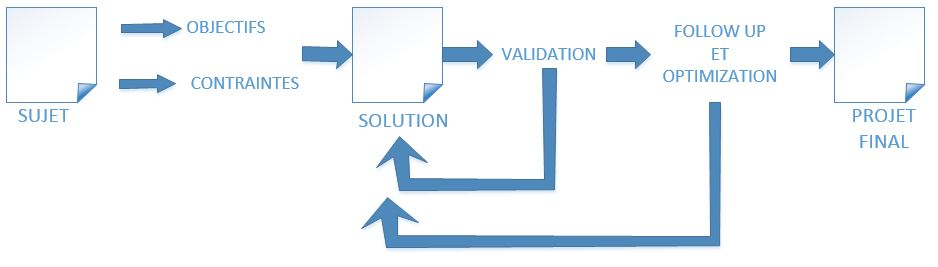
\includegraphics[width=15cm]{./diagrama.JPG}
		\caption{Méthodologie de projet}
		\label{fig:diagrama}
	\end{center}
\end{figure}



\vspace{20pt}
Le diagramme contient des objets (sujet, solution, projet final), éléments dérivés (objectifs, contraintes) et actions (valider, optimiser). On discutera brièvement toutes ses relations.
\begin{itemize}
	
\item Sujet : Document de spécification des besoins du client. Ordinairement ce document est composé par l’équipe avec le client, dans le cas des Olympiades il est déjà prêt.
\item 	Objectifs et contraintes : L’objectif est simplement ce que doit être atteint, décrit de manière simple et vérifiable. Les contraintes sont des limites que la solution doit respecter. Les deux sont dérivés du sujet, mais l’équipe doit ajouter contraintes supplémentaires afin de diminuer l’espace de solutions.
\item 	Solution : Ce que respecte les contraintes et accomplit les objectifs. Dans le cas des Olympiades une solution est composée d’une simulation dans le logiciel Roboguide.
\item 	Validation : Action d’évaluer une solution supposée afin de déterminer si, en fait, elle respecte les contraintes et accomplit les objectifs.
\item 	Optimisation : Action de critiquer la solution courant et proposer une autre solution que peut avoir une meilleure performance par rapport à une mesure de performance (temps total, coût, espace occupé, consommation d’énergie, etc.). 
\item 	Projet Final : Document que contient la description de la solution, la consolidation du projet et l’argumentation de la raison pour laquelle une entreprise quelconque devrait payer pour la solution proposée.
\end{itemize}

\vspace{20pt}
Cela dit, c’est facile de comprendre le flux du projet :
\begin{enumerate}
	\item On dérive les objectifs et les contraintes à partir du sujet.
\item	On propose des contraintes et hypothèses supplémentaires et on propose une solution. 
\item	On valide la solution, en mettant à l’épreuve les hypothèses faites dans l’étape dernière. Si la solution proposée n’accomplit pas les objectifs ou ne respecte pas les contraintes il faut retourner à l’étape 2 et vérifier quelle hypothèse était fausse ou quelle contrainte était excessive.
\item	Si la solution est validée, on a déjà une solution que marche. Dans cette étape il faut analyser la solution et proposer des améliorations, ou des solutions alternatives. Si on est satisfait avec la solution courant on passe à l’étape finale, autrement on retourne à l’étape 2 en proposant une autre solution.
\item	Dans cette étape il faut documenter la solution et la présenter en détail, avec des images et des chiffres, dans un document appelé projet final.

\end{enumerate}
